\chapter{Planung}

\label{chap:Planung}
Dieses Kapitel beschreibt die zu erwartende Probenmatrix und die Einzelheiten der Analyse, wie z.B. die Fällung der Matrix. Des Weiteren werden die notwendigen Grundlagen über Honig und HMF erläutert. Außerdem werden erste Berechnungen zur Erstellung einer Kalibriergeraden und den dazu nötigen Stammlösungen unternommen.

\section{Honig}
Honig besteht zum größten Teil aus Zucker. Zu etwa gleichen Teilen sind Fructose und Glucose mit je maximal 40\% enthalten. Andere Zucker wie Saccharose, Maltose und Melezitose sind je nach Zuckerart bis zu maximal 20\% enthalten. Da Honig jedoch ein Naturprodukt ist, kommen noch zahlreiche weitere Inhaltsstoffe darin vor. So enthält Honig Enzyme, die in den bieneneigenen Drüsen produziert werden. Drei der wichtigsten Enzyme sind die Invertase, die Amylase und die Glucoseoxidase. Invertase spaltet Saccharose in Glucose und Fructose, während die Amylase zur Spaltung der Stärke in Maltose dient. Glucoseoxidase wandelt in wässriger Lösung und in Verbindung mit Luftsauerstoff, Glucose in Wasserstoffperoxyd um und entwickelt damit eine antibakterielle Wirkung. Des Weiteren ist das in dieser Analyse bestimmte Hydroxymethylfurfural ein Bestandteil, der sich bei der Zersetzung von Fructose unter Wärme und Säureeinfluss bildet. Im Spurenbereich finden sich noch Vitamine, Hormone und Mineralstoffe im Honig. Außerdem kann die Aminosäure Prolin darin nachgewiesen werden. Der Gehalt beträgt je nach Reifegrad zwischen 250 und 550mg/kg.\\
Honig ist leicht sauer, sein pH-Wert liegt meist zwischen 3,2 und 5,4. Ursache dafür sind im Honig vorkommende organische Säuren. Hauptsächlich sind dies Ameisensäure und Zitronensäure. Deren Geschmack mag vom hohen Zuckergehalt überlagert werden, trotzdem hat Honig korrosive Eigenschaften.\\
Liegt der Honig als Rohprodukt vor und wurde nicht gefiltert, sind in ihm auch noch einige feste Bestandteile enthalten wie Pollenkörner, Pilzsporen, Algen und auch tierische Bestandteile wie Bienenhaare. Zuletzt findet sich auch ein nicht unerheblicher Anteil an Wasser im Honig. Dieser kann zwischen 15 und 19\% betragen. Ist der Wassergehalt erhöht, kann es zur Gärung kommen und der Honig verdirbt. Ist er zu niedrig kristallisiert der Zucker aus und der Honig wird inhomogen.\\
Alle diese Bestandteile können die photometrischen Analyse behindern. Sie können entweder die gesamte Lösung trüben oder eine Absorptionsbande im Messbereich bei 550nm aufweisen. Deshalb werden die meisten Matrixbestandteile vorher abgetrennt.~\cite{LWG}
\begin{figure}[htbp]
    \centering
        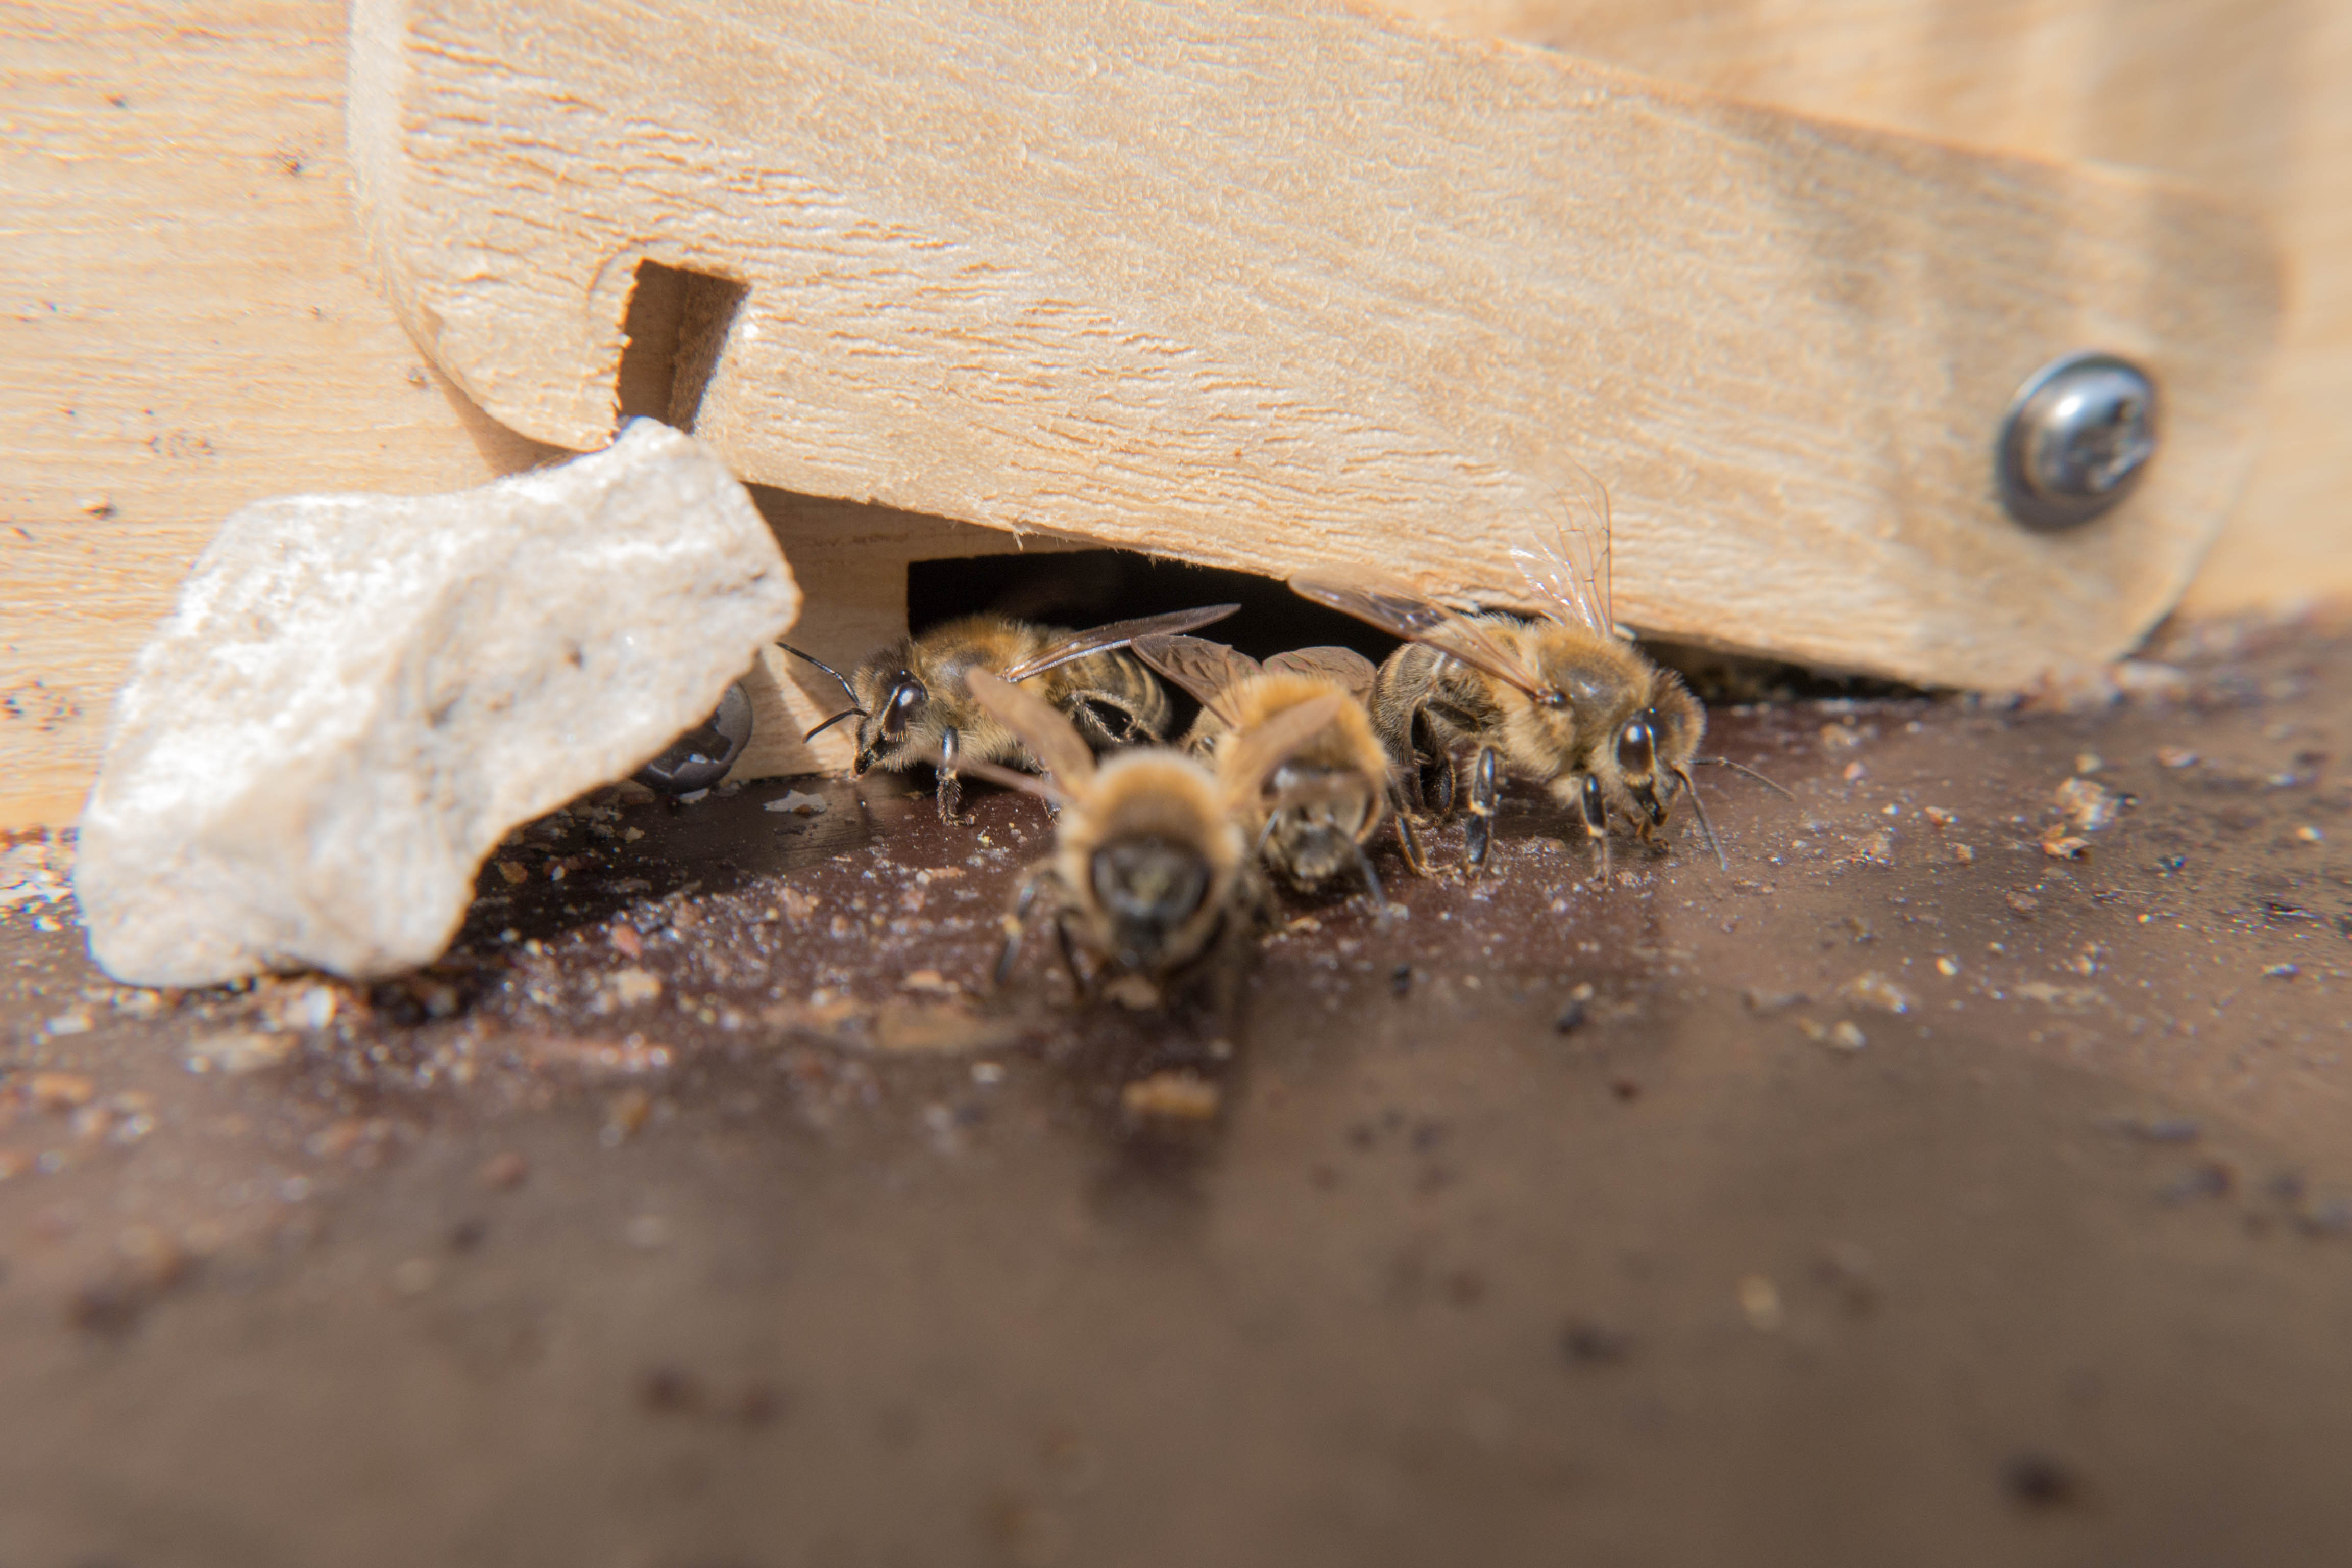
\includegraphics[width=1.00\textwidth]{../Bilder/P1050729.jpg}
    \caption{Bienen \cite{Bienen}}
    \label{fig:Bienen}
\end{figure}


\section{Bildung von HMF}

Wird Honig über lange Zeit gelagert oder hohen Temperaturen ausgesetzt, so bildet sich aus der enthaltenen Fructofuranose unter Wasserabspaltung Hydroxymethylfurfural.~\cite{HMF} Dies verdeutlicht die folgende Reaktionsgleichung \ref{fig:HMFEntstehung}. 
  
\begin{figure}[htbp]
    \centering
        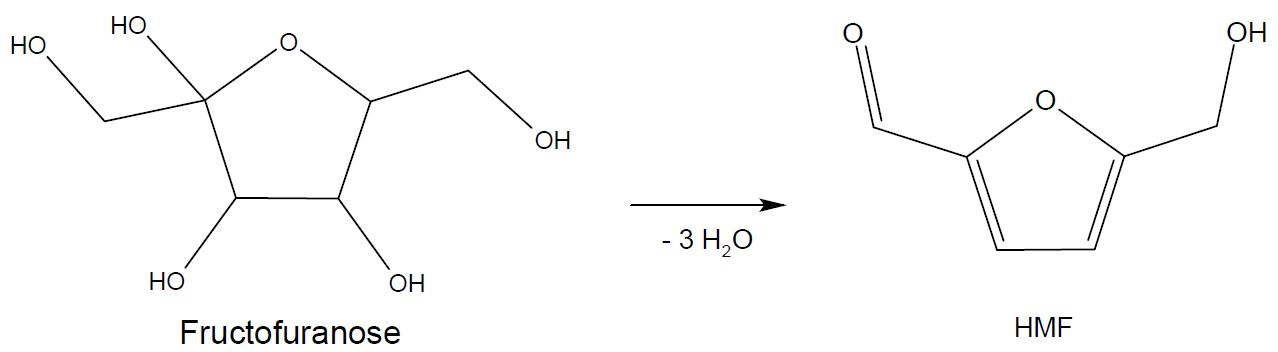
\includegraphics[width=1.00\textwidth]{../Bilder/HMFEntstehung.JPG}
    \caption{Reaktionsgleichung: Bildung von HMF aus Fructofuranose}
    \label{fig:HMFEntstehung}
\end{figure}

\section{Nachweis nach Winkler}

O. Winkler veröffentlichte im September 1955 in der ``Zeitschrift für Lebensmittel-Untersuch-ung und -Forschung'' einen Bericht über eine neue Methode HMF spektroskopisch in Honigen nachzuweisen. Dieser Nachweis basiert auf Furfurol-Farbstoffen, die von Boehm und Grohnewald beschrieben wurden und auf der von Akabori dargestellten Reaktion von Furfuraldehyden mit Barbitursäure und Anilin. Winkler ersetzte das Anilin durch p-Toluidin, ein kernsubstituiertes Derivat, das die gleiche Reaktion mit HMF und Barbitursäure zeigt. Durch Zugabe von Eisessig in die isopropanolische p-Toluidinlösung konnte die Empfindlichkeit der Reaktion gesteigert werden. P-Toluidin wird als potentiell krebserzeugend eingestuft und muss deshalb mit größter Vorsicht im Abzug und mit der nötigen persönlichen Schutzausrüstung gehandhabt werden.\\
Der entstehende rote Farbstoff, der in der folgenden Reaktionsgleichung \ref{fig:Farbreaktionsgleichung2} dargestellt ist, absorbiert bei 550nm das sichtbare Licht. Drei bis vier Minuten nach Zugabe des letzten Reaktionsmittels erreicht der Farbstoff seine maximale Konzentration. Danach setzt der Zerfall ein. Nach O. Winkler ist die Linearität der Messung zwischen 5 und 300ppm HMF gegeben.~\cite{Winkler}

\begin{figure}[htbp]
    \centering
        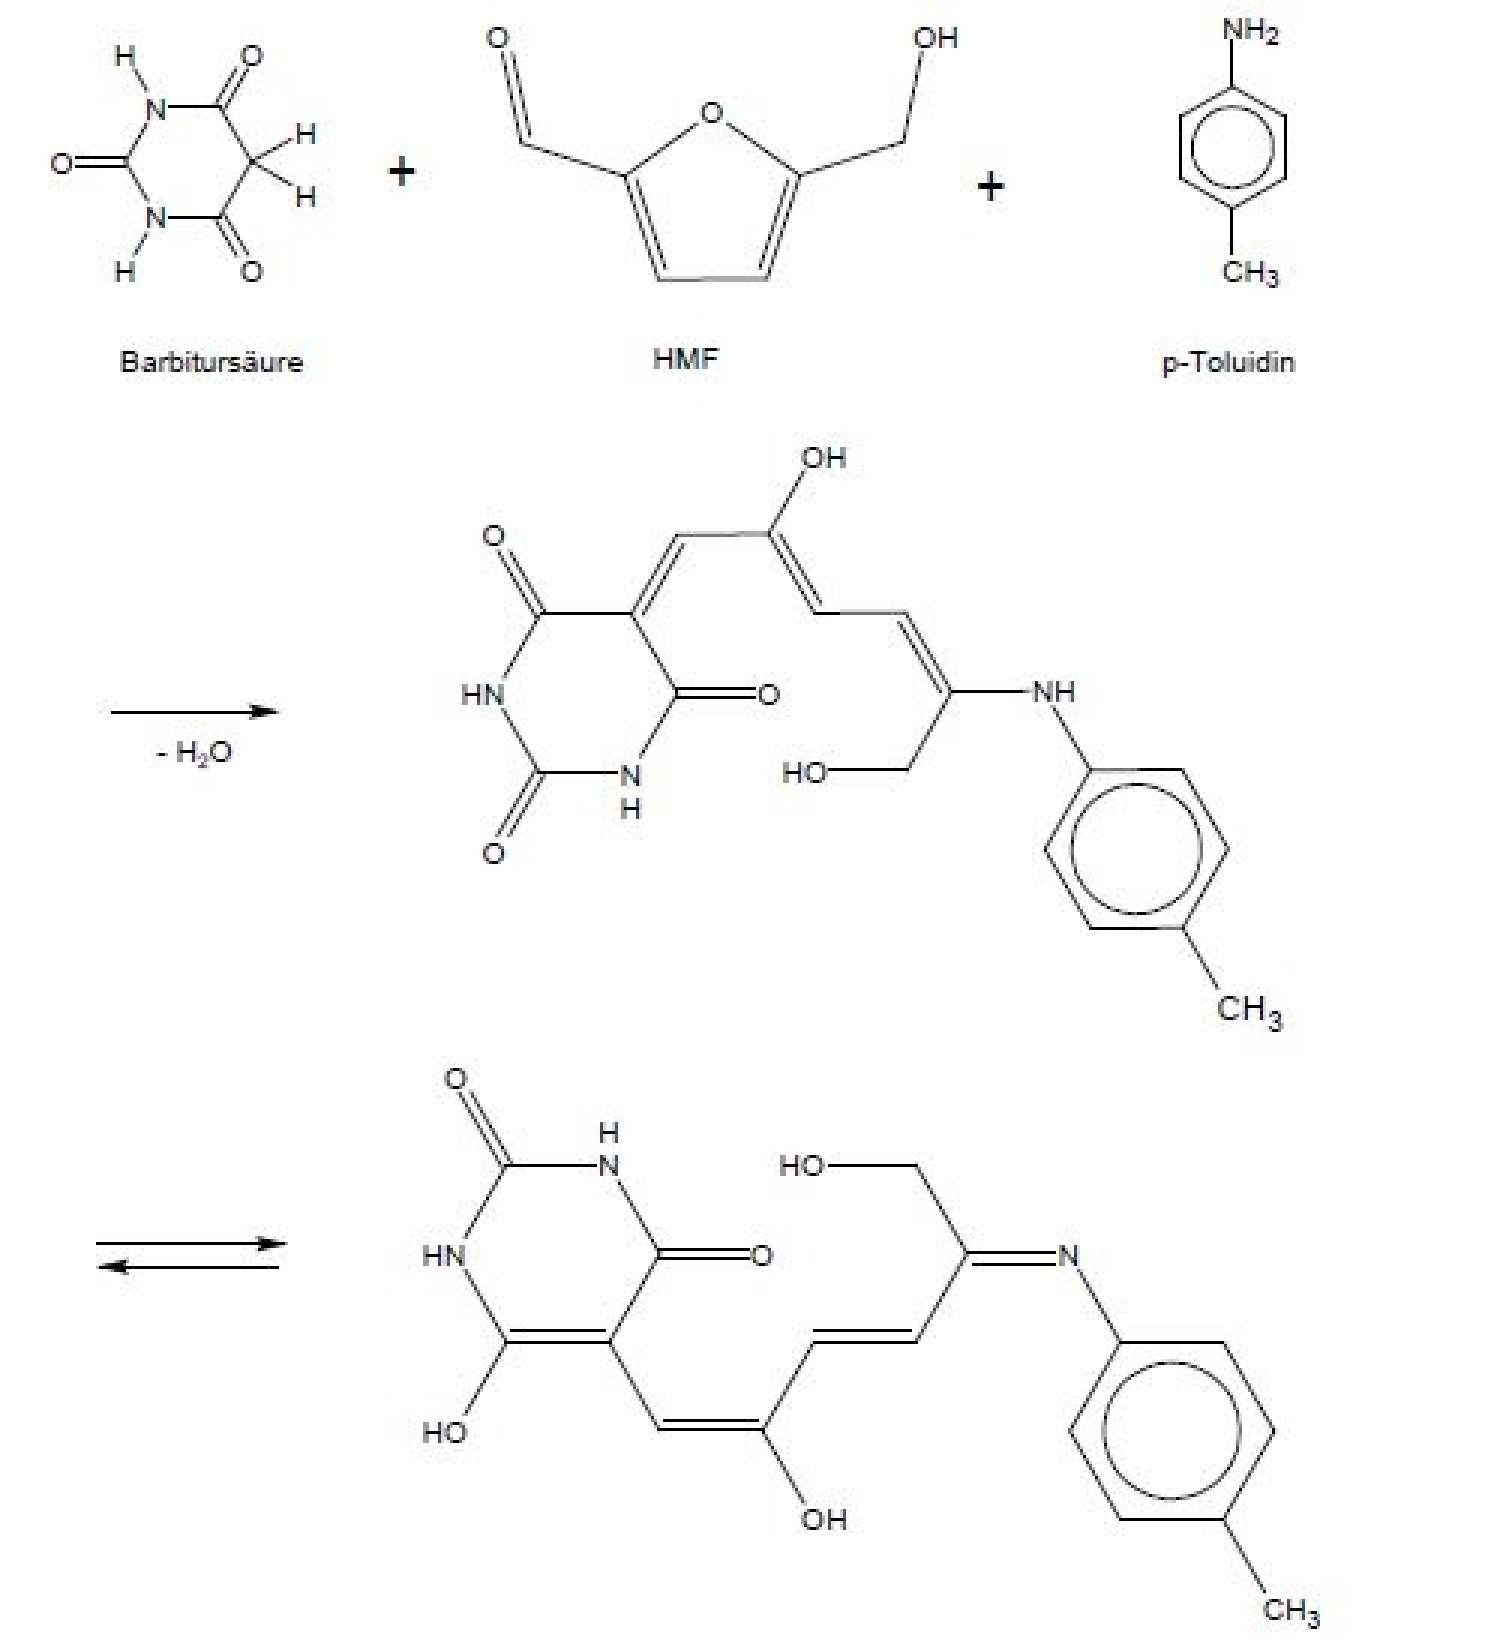
\includegraphics[width=1.00\textwidth]{../Bilder/Farbreaktionsgleichung2.pdf}
    \caption{Reaktionsgleichung: Bildung des Farbstoffs aus HMF}
    \label{fig:Farbreaktionsgleichung2}
\end{figure}

\section{Alternative Nachweismethoden}

Neben dem HMF-Nachweis nach WINKLER gibt es noch weitere Methoden um HMF in zuckerhaltigen Produkten nachzuweisen.\\
Es gibt zum Beispiel die Möglichkeit das HMF mit Diethylether aus der Probe zu extrahieren und mit einer Resorcinlösung, auch Seliwanoff-Reagenz genannt, als roten Farbstoff sichtbar zu machen. Da Resorcin auch mit der vorhandenen Fructose reagiert, ist für einen korrekten Nachweis eine saubere Extraktion unbedingt notwendig. Allerdings sind sowohl Resorcin als auch Diethylether gesundheitsschädlich und der Versuch muss im Abzug durchgeführt werden.~\cite{Resorcinnachweis} Hierbei handelt es sich um den sogenannten Fieheschen Nachweis.~\cite{Winkler}\\
Weiterhin zeigt HMF in wässriger Lösung bei 282nm ein Absorptionsmaximum. Über diesen und zwei weitere Messpunkte bei 245 und 325nm lässt sich nach Schou und Abildgaard der HMF-Gehalt in einer Probe berechnen. Allerdings absorbiert z.B. Honig bei diesen Wellenlängen durch seine Matrixbestandteile ebenfalls Licht. Dies verfälscht das Messergebnis. Durch Zugabe der Carrez-Lösungen I und II können die störenden Bestandteile zu einem Großteil entfernt werden und das Ergebnis verbessert werden.~\cite{Winkler}
Alternativ kann HMF auch per Gaschromatographie oder HPLC bestimmt werden. Hierfür müssen die Proben in einer säulengängigen Form vorliegen und die Methoden für eine Quantifizierung mit einem HMF-Standard kalibriert werden.~\cite{Patent}
Alle hier genannten HMF-Nachweise sind mit hohem chemischem und apparativem Aufwand verbunden. Außerdem sind die verwendeten Chemikalien gesundheitsschädlich oder sogar giftig und müssen deshalb mit größter Vorsicht gehandhabt werden. Aus diesen Gründen wurde von Merck ein einfacher Schnelltest entwickelt. Dieser erfolgt mit Teststäbchen, die mit zwei Reaktionslösungen belegt sind. Die Stäbchen müssen nur in die Probe eingetaucht und dann in einem Reflektometer vermessen werden. Hierbei erfolgt die Farbreaktion auf dem Teststäbchen. Das Gerät kann HMF-Konzentrationen zwischen 1 und 60mg/L erfassen. Höher konzentrierte Proben müssen verdünnt und das Messergebnis mit dieser Verdünnung verrechnet werden. Die Farbreaktion ist zeitabhängig, deshalb muss auch hierbei die Reaktionszeit genau eingehalten werden.~\cite{Merck}

\section{Bedeutung von HMF}
In den 1950er Jahren wurde HMF erstmals in Lebensmitteln nachgewiesen. Es besitzt kein relevantes toxisches Potential. Die lethale Dosis bei oraler Einnahme für Ratten beträgt 3100mg/kg. Jedoch ist die karzinogene Wirkung von HMF weitestgehend unklar. Zwar kann aus bisher vorliegenden Studien keine Relevanz bezüglich krebserzeugender oder erbgutschädigender Wirkung beim Menschen festgestellt werden, jedoch ist die Bedeutung der Stoffwechselabbauprodukte und deren Wirkung bei der Entstehung von Darmkrebs nicht restlos aufgeklärt. Eine kurzzeitig angenommene krebsvorbeugende Wirkung konnte ebenfalls nicht bestätigt werden.
\\
Honig enthält auch bei hohen Konzentrationen im Vergleich zu anderen Lebensmitteln relativ wenig HMF. Nach Daten des Bundesinstituts für Risikobewertung hat Honig einen mittleren HMF-Gehalt von 9,1mg/kg. Zum Vergleich besitzt Mehrfruchtnektar einen mittleren Gehalt von 40,9mg/kg und Saft aus Trockenpflaumen sogar einen mittleren Gehalt von 1022,1mg/kg. Der Massenanteil an HMF in Honig ist somit primär der Indikator für Frische und die korrekte Lagerung. So gelten für Honig in Deutschland verschiedene Bestimmungen, die den maximalen Massenanteil an HMF vorgeben. Nach der deutschen Honigverordnung ist in deutschem Honig maximal 40mg/kg HMF zulässig, sonst ist dieser Honig als Industriehonig oder Backhonig zu kennzeichnen. In Honig aus tropischen Regionen ist sogar ein Gehalt von 80mg/kg noch erlaubt. Deutlich strenger sind die Kriterien, die der Deutsche Imkerbund an Honige anlegt, die das Gütesiegel ``echter deutscher Honig'' tragen wollen. Hierfür liegt die Obergrenze für HMF bei 15mg/kg und für niedrig enzymatischen Honig sogar nur bei 5mg/kg.
\\
Eine direkte Verwendung findet HMF als Bestandteil von Raucharoma Lebensmitteln. Jedoch wird HMF derzeit neu betrachtet und eventuell neu bewertet.~\cite{BfR}

\section{Funktionsweise eines UV/VIS-Spektrometers}

\begin{figure}[htbp]
    \centering
        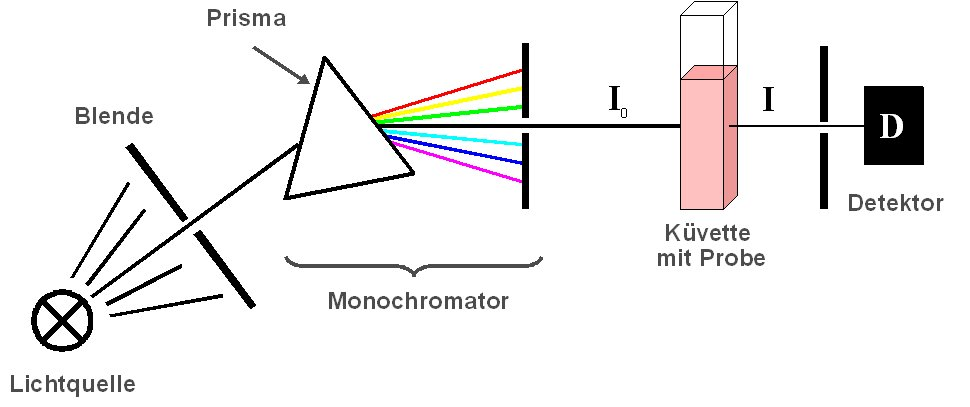
\includegraphics[width=1.00\textwidth]{../Bilder/Einstrahlspektrometer.jpg}
    \caption{Schematischer Aufbau eines Einstrahl-Absorptionsspektrometers \cite{Schema}}
    \label{fig:Einstrahlspektrometer}
\end{figure}

Die UV/VIS-Spektrometrie gehört zur Absorptionsspektroskopie. Dabei wird die Konzentration
eines Lösungsbestandteils (= Analyt) in einer optisch klaren Lösung über die Absorption
eines möglichst monochromatischen Lichtstrahls bestimmt.\\
Aus dem polychromatischen Licht einer Lichtquelle wird mittels einer Blende ein dünner
Lichtstrahl abgetrennt und auf ein Prisma gelenkt. Dort wird er in einzelne monochromatische
Lichtstrahlen aufgetrennt. Ein Lichtstrahl einer bestimmten Wellenlänge wird
durch eine Küvette, die mit der Probelösung gefüllt ist, geleitet. Ein Teil des Lichtstrahls wird
durch die Probe absorbiert. Das restliche austretende Licht wird detektiert und die Extinktion
daraus berechnet.
\begin{figure}[htbp]
    \centering
        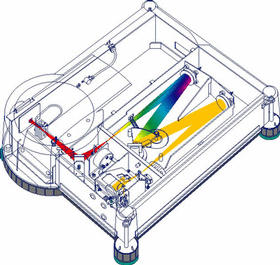
\includegraphics[width=1.00\textwidth]{../Bilder/AufbauSpektrometer.jpg}
    \caption{Schematischer Aufbau Varian Cary® 50 Scan UV/VIS-Spektrometer \cite{UV-VIS}}
    \label{fig:AufbauSpektrometer}
\end{figure}

Das UV-VIS Spektrometer Varian Cary® 50 benutzt eine Xenon-Blitzlampe als Lichtquelle. Das Instrument wird direkt über einen Computer mit der Cary Win UV-Software gesteuert. 
\begin{figure}[htbp]
    \centering
        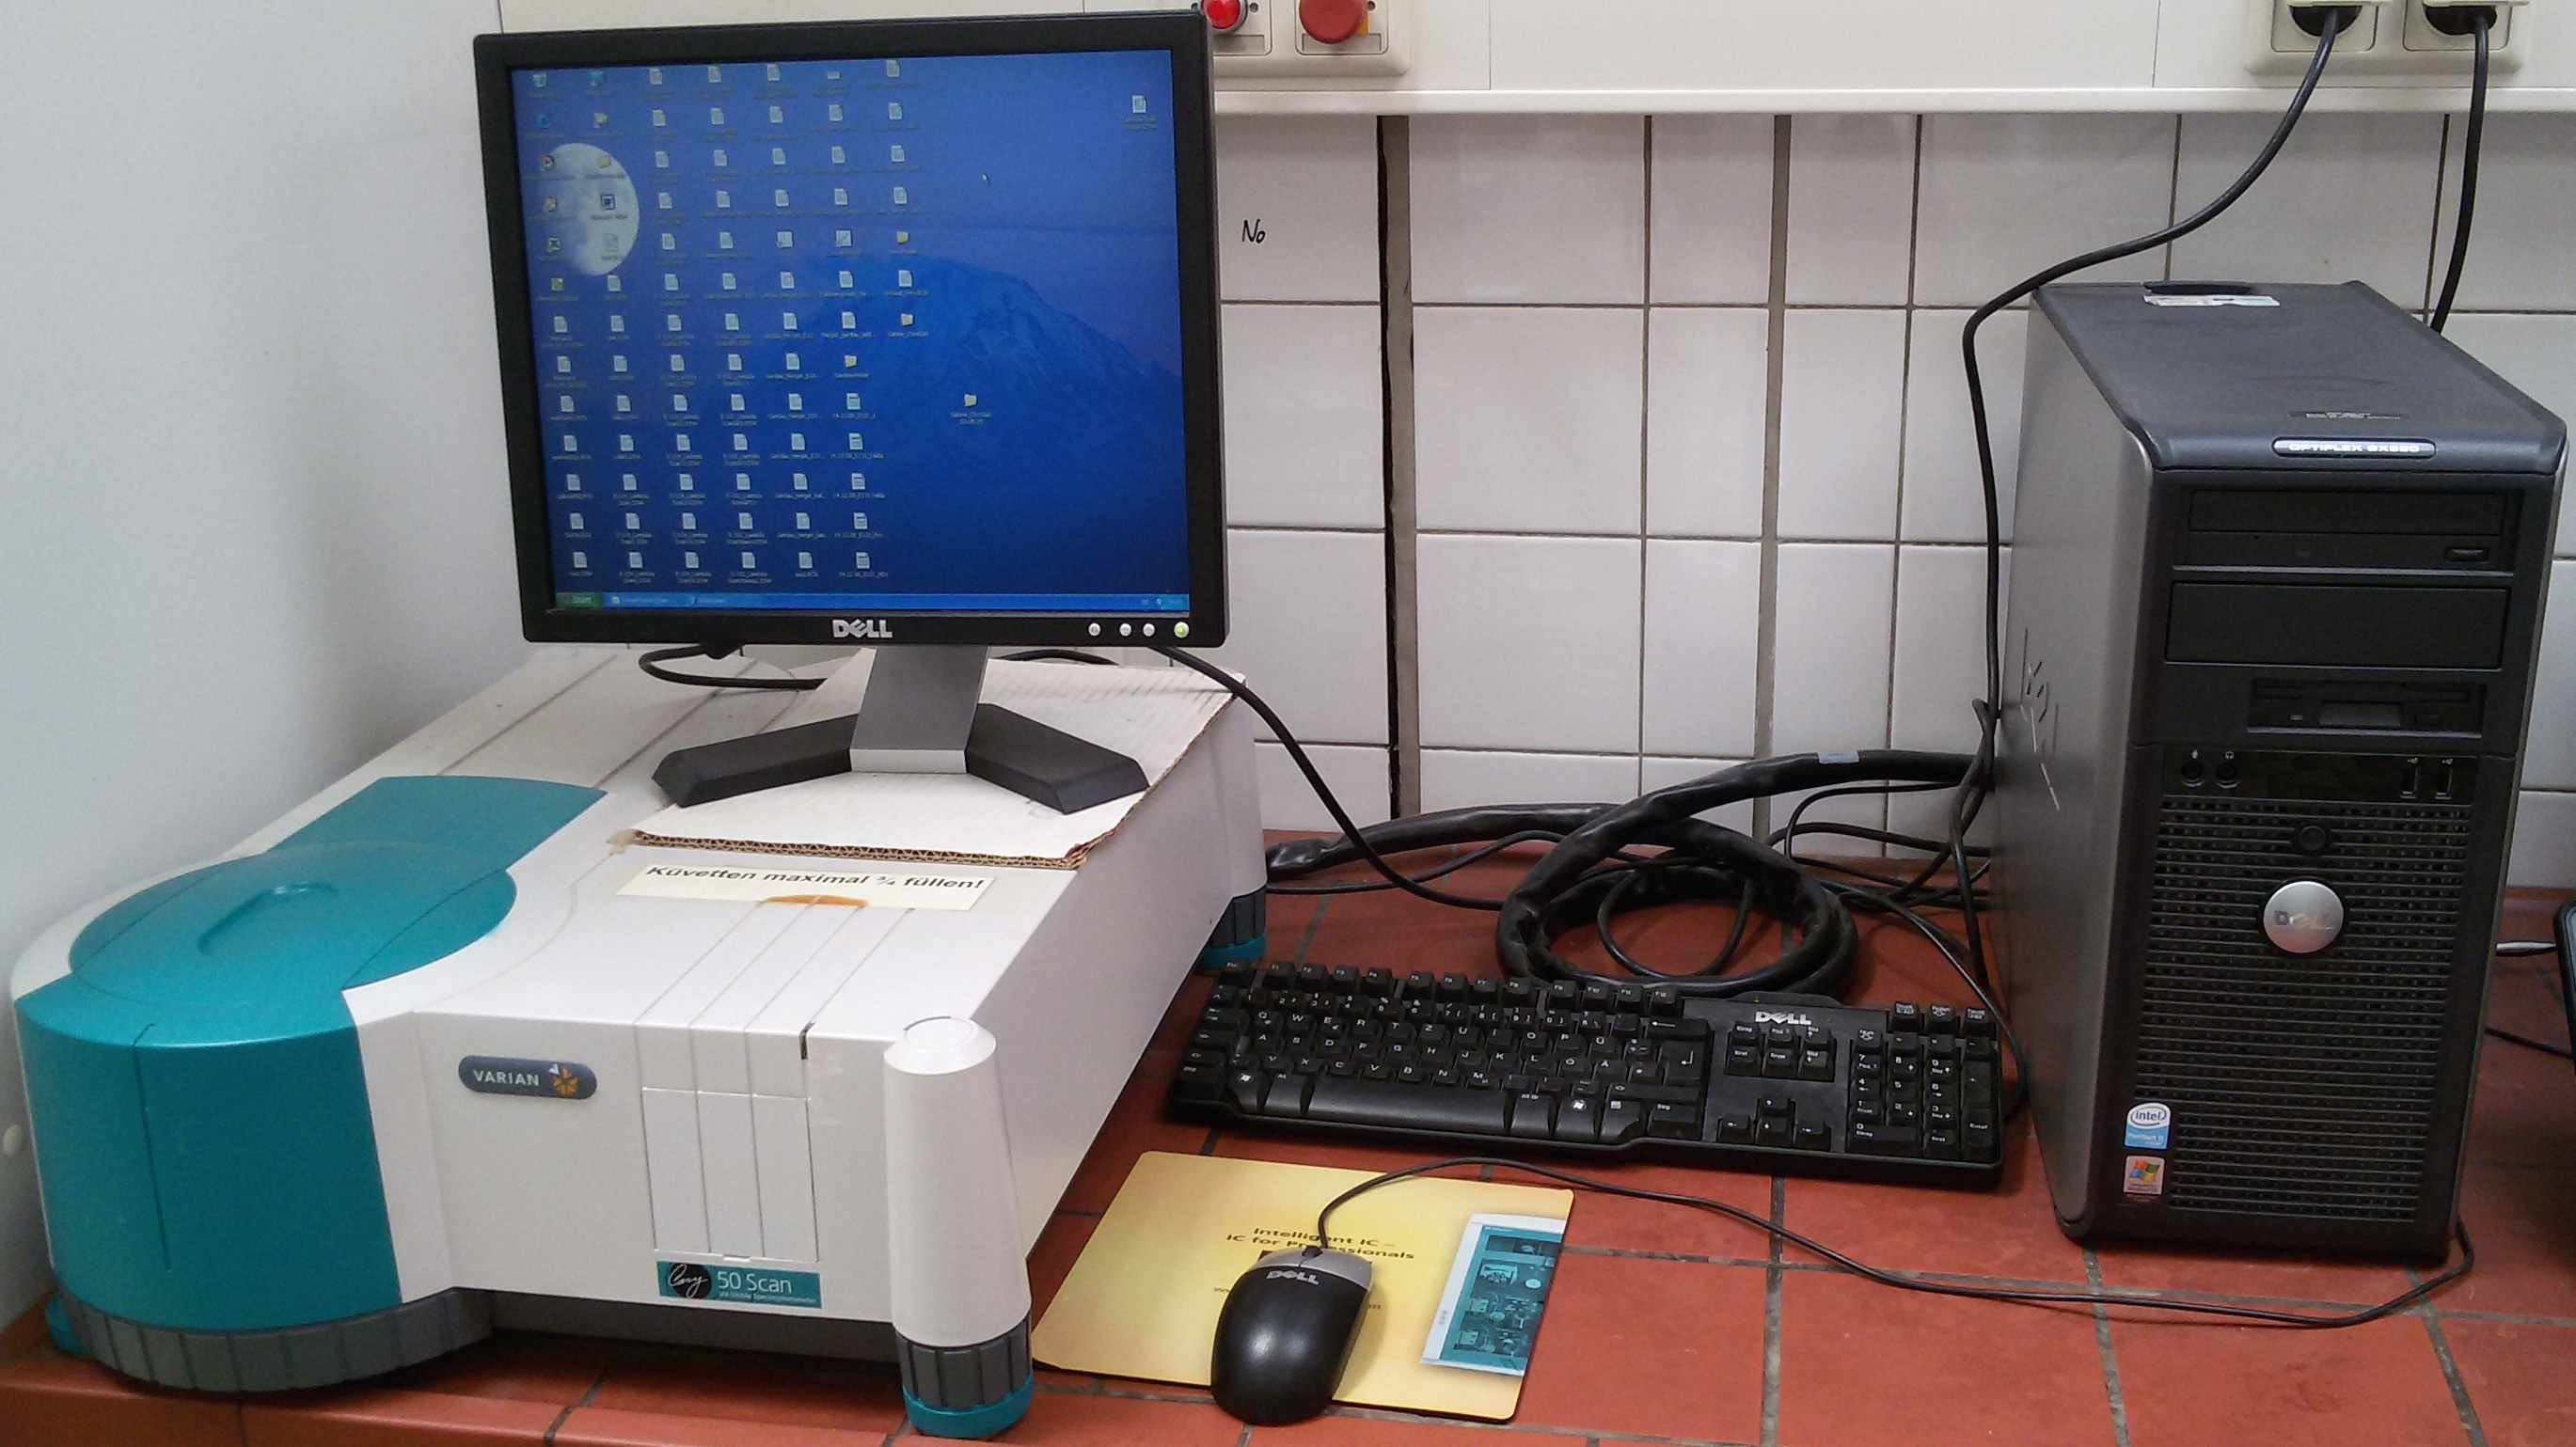
\includegraphics[width=1.00\textwidth]{../Bilder/20150504_140611.jpg}
    \caption{Varian Cary® 50 Scan UV/VIS-Spektrometer}
    \label{fig:Spektrometer}
\end{figure}

\section{Funktion Carrez-Lösung}
Da die Honiglösung noch viele trübende Bestandteile enthält, muss sie mit der Carrez-Klärung von Kolloiden getrennt werden. Dazu wird eine Lösung aus gelbem Blutlaugensalz (Carrez I) und eine Lösung aus Zinkacetat (Carrez II) verwendet. Beide Lösungen müssen zu gleichen Teilen der Probelösung zugegeben werden. Dabei entsteht Kalium-Zink-hexacyanoferrat(II) $(K_{2}Zn_{3}[Fe(CN)_{6}]_{2})$, das die meisten kolloiden Trübstoffe aus der Lösung entfernt. Nach zahlreichen Versuchen von O. Winkler findet eine Absorption des entstehenden Farbstoffs mit dem Klärmittel nicht statt. Durch Filtration können die ausgefallenen Bestandteile abgetrennt und verworfen werden. Das klare Filtrat kann weiter verarbeitet werden.~\cite{Winkler}

\section{Organisation des Abschlussprojektes}
Während der Recherchen zur Durchführung unseres Abschlussprojektes entdeckten wir, dass die beiden Reaktionslösungen (p-Toluidinlösung und Barbitursäure) in der benötigten Konzentration im Chemikalienhandel erhältlich sind. Über die Chemikalienbeschaffung der BASF SE konnten sowohl der benötigte HMF-Standard als auch die beiden Reaktionslösungen bestellt werden. Somit entfällt das Ansetzen der beiden Lösungen während des Praktikums. Der Hersteller der p-Toluidinlösung konnte keine Angabe zur Haltbarkeit nach Öffnung der Flasche machen. Die selbst angesetzte Lösung wäre nur drei Tage haltbar gewesen. Die restlichen Chemikalien stellte die Berufsschule zur Verfügung.

\begin{figure}[tbp]
    \centering
        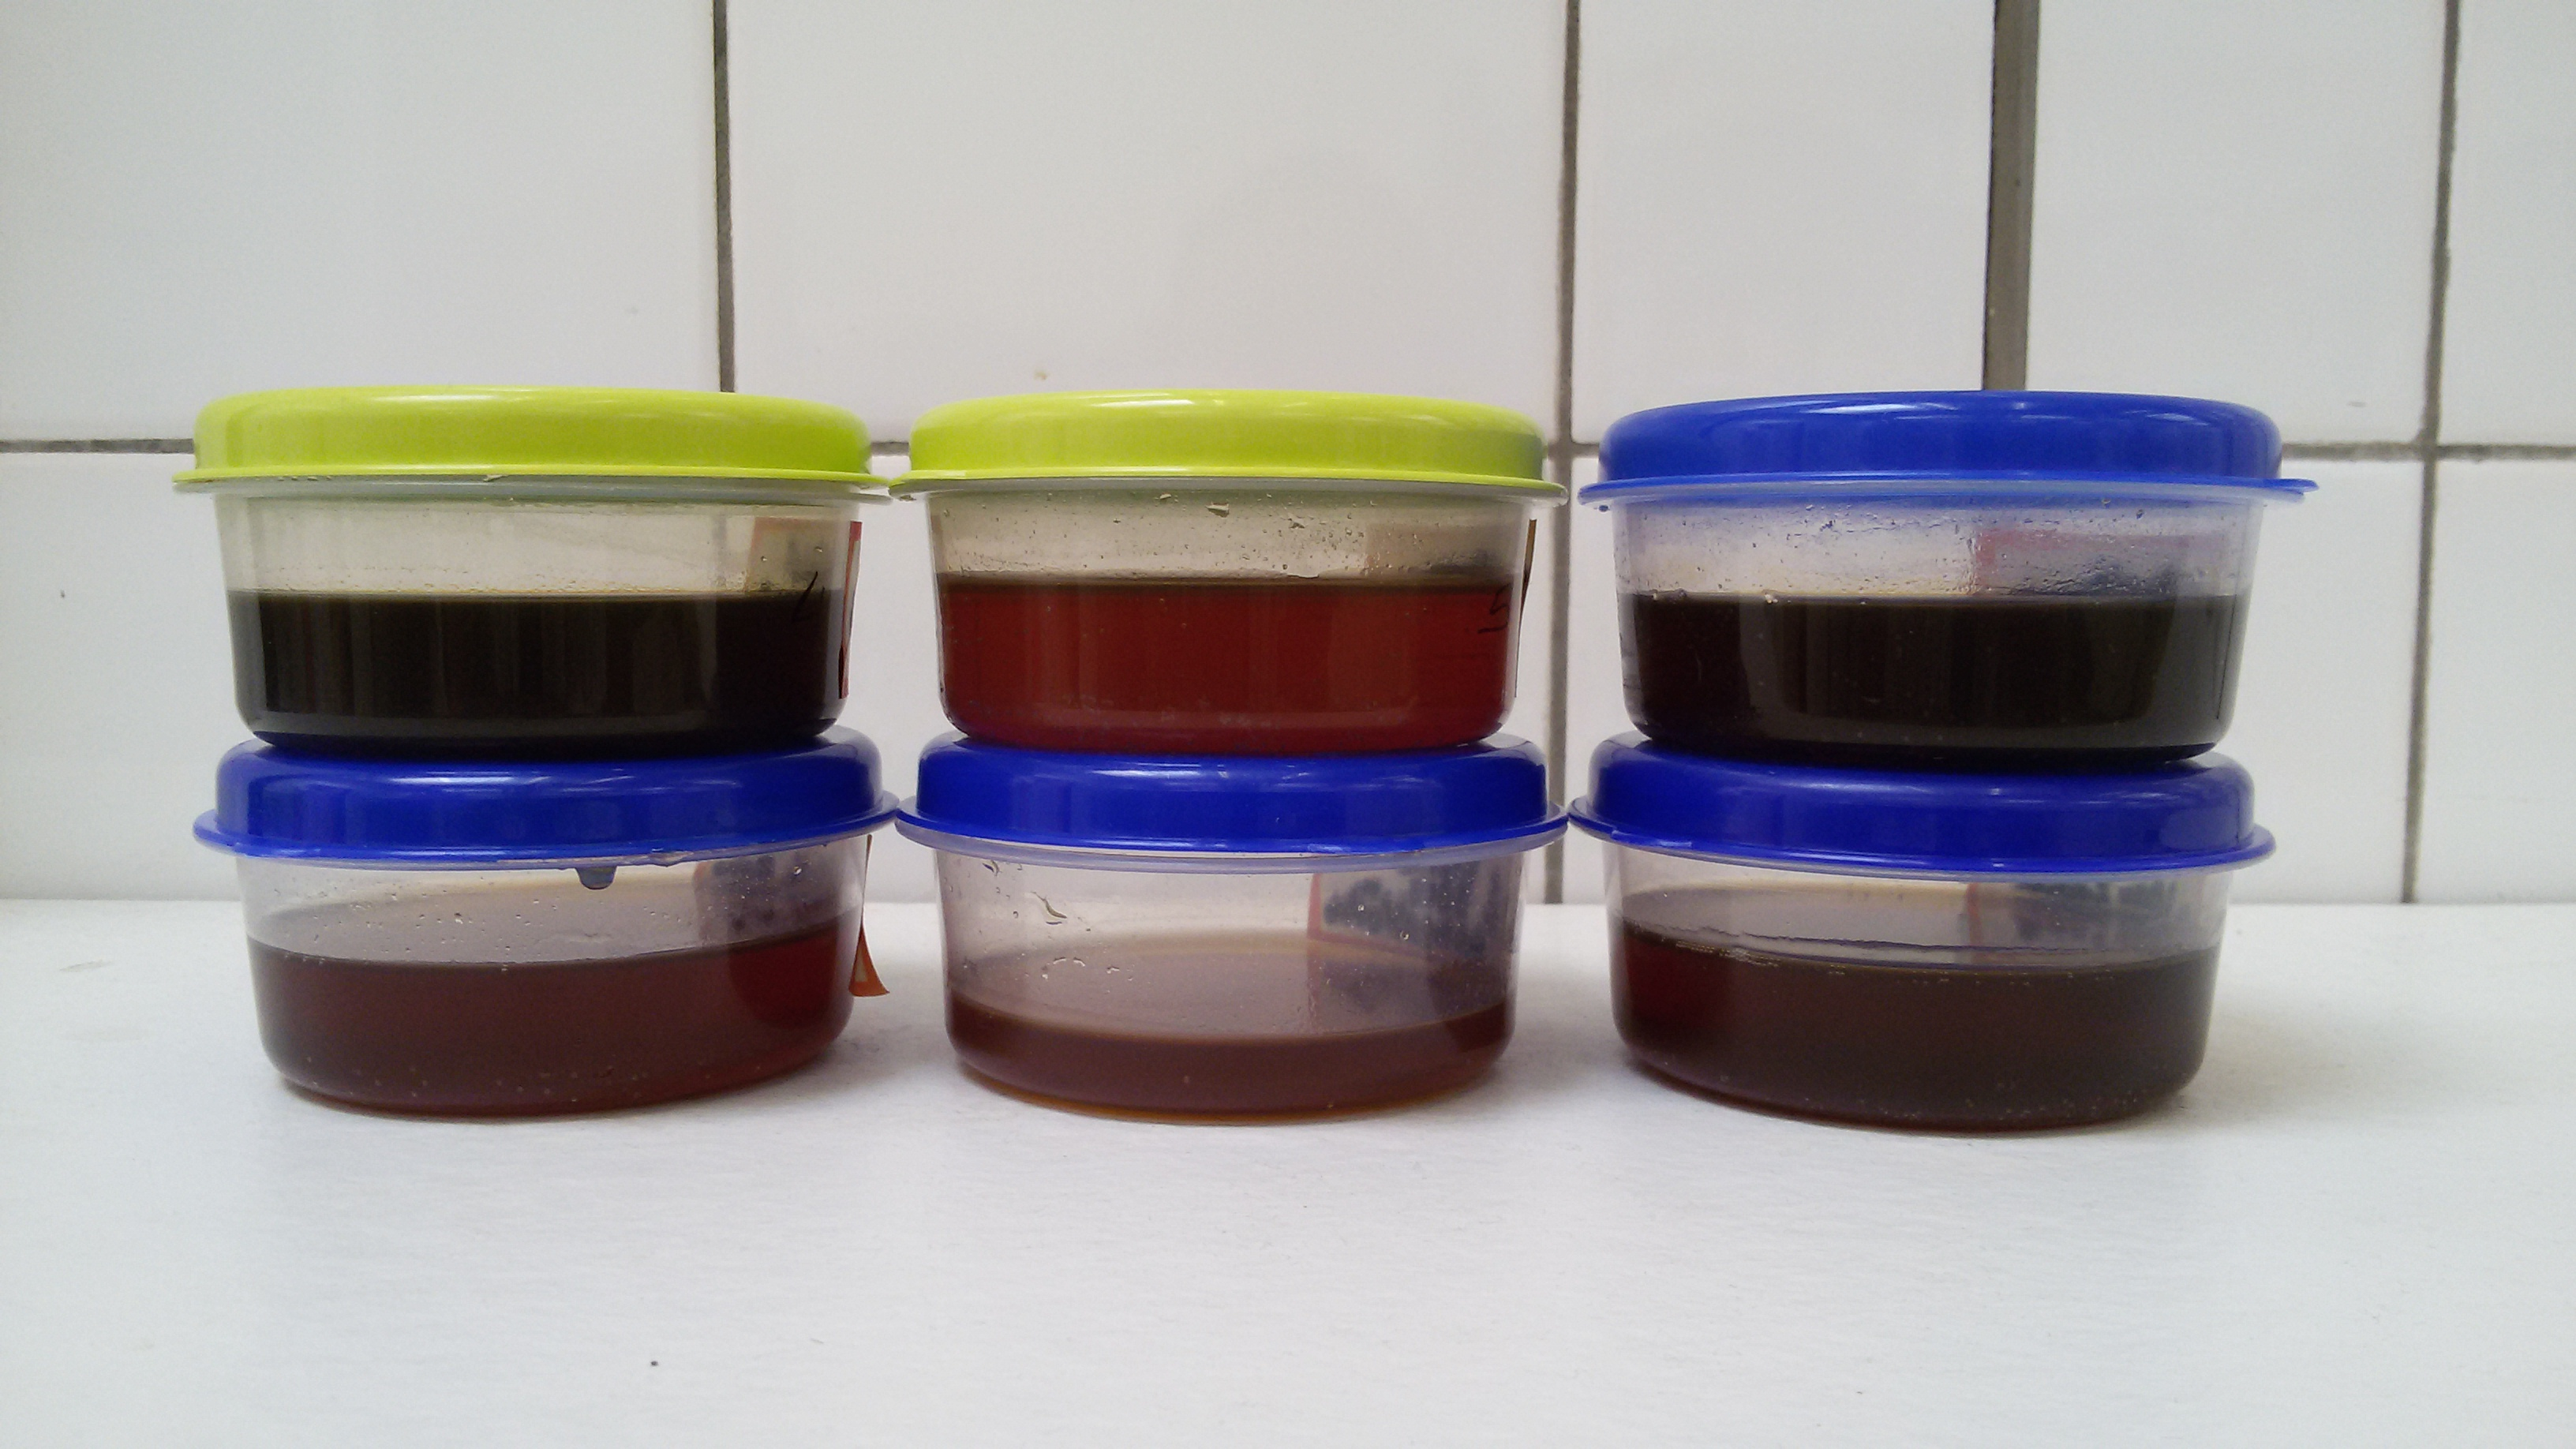
\includegraphics[width=1.00\textwidth]{../Bilder/20150504_141528.jpg}
    \caption{Honigproben für Lagertest}
    \label{fig:Lagertest}
\end{figure}

Zehn Tage vor dem zweiten Praktikumstag wurden die zugekauften Chemikalien im Chemikalienkühlschrank der Biologie in der BBSN Ludwigshafen verwahrt. Am gleichen Tag wurden auch die sechs Honigproben für den Lagertest abgefüllt. Sie wurden in einem Wärmeschrank der Biologie bei einer Temperatur von $60^\circ$ C gelagert.\\
Für die Durchführung des Abschlusspraktikums wurden anderthalb Praktikumstage angesetzt. Auf Grund von Problemen während des Praktikums wurde ein zusätzlicher Tag benötigt. \\
Für die vier Stunden des ersten Praktikumstages wurde das Ansetzen der beiden Carrez-Lösungen, eine erste Probemessung mit einer Honigprobe ohne und mit Temperaturlagerung und das Erstellen der Kalibriergeraden vorgesehen.\\
Am zweiten Praktikumstag sollten die Proben vermessen werden. Da hierbei erkannt wurde, dass der Farbstoff nach einiger Zeit zerfällt, wurde ein weiterer Praktikumstag eingeplant.\\
Während des dritten Tages wurde die Kalibrierung wiederholt und eine Sechsfachanalyse, sowie eine Aufstockung einer Honigprobe mit HMF durchgeführt.\\

\section{Berechnungsgrundlagen}
Für die Berechnung der notwendigen Kalibrierlösungen berücksichtigen wir, dass in den Versuchen von WINKLER die Extinktion von HMF zwischen 5 - 300mg/kg einen linearen Verlauf aufweist. Um die Möglichkeit eines zufälligen Wägefehlers zu minimieren, werden zwei Stammlösungen mit verschiedenen Konzentrationen angesetzt. Auf Grund der benötigten Kalibrierung mit 5mg/kg, müssen die Stammlösungen noch entsprechend verdünnt werden. Für die kleinste und größte Kalibrierung werden folgende Mengen HMF benötigt:

    \[w[mg/kg]=\frac{ m(HMF) }{ m(Gesamt) }\]
    
Die Formel wird nach m(HMF) umgestellt.

    \[m(HMF)=w[mg/kg]*m(Gesamt)\]
    
Für 5mg/kg bedeutet dies:
    
    \[0,05mg=5mg/kg*0,01kg\]
    
Und für 300mg/kg:

    \[3,00mg=300mg/kg*0,01kg\]
    
Alle Massenanteile beziehen sich auf eine ideale Einwaage von 10,00g und ein Endvolumen von 50ml.
Da die Kalibriergerade der Software die Massenkonzentration in mg/L ausgibt, werden die Gehalte zusätzlich entsprechend umgerechnet:

\[\beta=\frac{ m(HMF) }{ V }\]

Das bedeutet bei 5mg/kg:

\[1mg/L=\frac{ 0,05mg }{ 0,05L }\]

Und wieder für 300mg/kg:

\[60mg/L=\frac{ 3,00mg }{ 0,05L }\]

Wir erwarten vor allem Gehalte zwischen 5 und 100mg/kg HMF in unseren Proben, deshalb liegen die meisten unserer Kalibrierpunkte eher in diesem Konzentrationsbereich.
In Tabelle \ref{tab:Stammlösungen} sind die Daten für die Stammlösungen aufgelistet:

\begin{table}[htbp]
    \centering
    \caption{Stammlösungen}
        \begin{tabular}{l|c|c|l}
            Bezeichnung & m(HMF) in mg & Konzentration in mg/L & Bemerkung\\
            \hline
            Stammlösung 1 & 50 & 5000  & in 10ml Messkolben\\
            \hline
            Stammlösung 1.1 & 5 & 50 & 1ml SL1 in 100ml\\
            \hline
            Stammlösung 2 & 150 & 15000 & in 10ml Messkolben\\
            \hline
            Stammlösung 2.1 & 15 & 150 & 1ml SL2 in 100ml\\
        \end{tabular}
        \label{tab:Stammlösungen}
\end{table}

Aus den Stammlösungen werden die in der folgenden Tabelle \ref{tab:IdealeKalibrierfaktoren} eingetragenen Faktoren hergestellt:

\begin{table}[htbp]
    \centering
    \caption{Ideale Kalibrierfaktoren}
        \begin{tabular}{L{0.15\linewidth}|C{0.15\linewidth}|C{0.17\linewidth}|C{0.17\linewidth}|L{0.22\linewidth}}
            Bezeichnung & m(HMF)\newline in mg & Konzentration\newline in mg/L & Massenanteil\newline in mg/kg & Bemerkung\\
            \hline
            Faktor 1 & 0,05 & 1,00  & 5 & 1ml SL1.1 in 50ml\\
            \hline
            Faktor 2 & 0,15 & 3,00  & 15 & 1ml SL2.1 in 50ml\\
            \hline
            Faktor 3 & 0,25 & 5,00  & 25 & 5ml SL1.1 in 50ml\\
            \hline
            Faktor 4 & 0,50 & 10,00 & 50 & 10ml SL1.1 in 50ml\\
            \hline
            Faktor 5 & 1,50 & 30,00 & 150 & 10ml SL2.1 in 50ml\\
            \hline
            Faktor 6 & 3,00 & 60,00 & 300 & 20ml SL2.1 in 50ml\\
        \end{tabular}
        \label{tab:IdealeKalibrierfaktoren}
\end{table}

Allen diesen Konzentrationen liegen ideale Berechnungen zugrunde. Die wirklichen Einwaagen sind im Kapitel~\ref{chap:Durchführung} zu finden.
